\documentclass[border=20pt]{standalone}

\usepackage{tikz}
\usetikzlibrary{calc,angles, quotes}

\begin{document}

    
    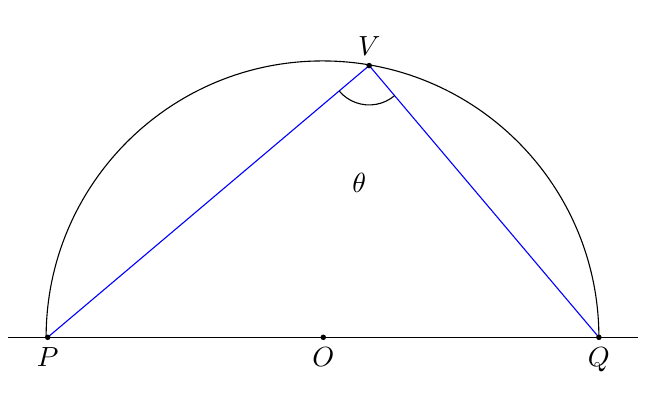
\begin{tikzpicture}

      \def \radius{3.5}
      \coordinate (V) at ($(0,0)!\radius cm!rand*45:(0,\radius)$);
      
      \path (-\radius, 0) coordinate(P) -- 
                   coordinate[midway](O)
                   (\radius, 0) coordinate(Q);
      
      % Draw semicircle
      \draw (Q) arc(0:180:\radius1);
      \draw[shorten <=-5mm, shorten >=-5mm] (P) -- (Q);
      
      %draw an arc starting at [partway from V to Q], to[ partway from V to P]
      \draw [color=blue] (P)--(V)--(Q);
      \pic [draw, "$\theta$", angle eccentricity=3] {angle=P--V--Q};
      
      \node at (O) [below]  {$O$};
      \node at (P) [below]  {$P$};
      \node at (Q) [below]  {$Q$};
      \node at (V) [above]  {$V$};
      
      \foreach \p in {O,P,Q, V}{
        \fill (\p) circle (1pt);
      }\
      
    \end{tikzpicture}

\end{document}